\chapter{Umsetzung}
\label{ch:S5_Umsetzung}

\section{Erläuterung des Softwaretechnischen Entwurfs}

Für die Softwaretechnische Umsetzung wurden zunächst die Anforderungen an das Geogameframework in Kapitel \ref{ch4:s:Lösungen} sowie die gewählte Lösung aus Kapitel \ref{ch4:s:choosen_solution} im Detail evaluiert. Für die Umsetzung des Entwurfs wurde zunächst ein Entwurfs des Prozesses identifiziert, welcher die Geodaten aus OSM bis hin zur Darstellung im Beispielspiel darstellt. Eine Visualisierung ist in Abbildung \ref{img:ch5_img01_framework_progress} zu sehen.
\\\\

\begin{figure}[H]
\begin{center}
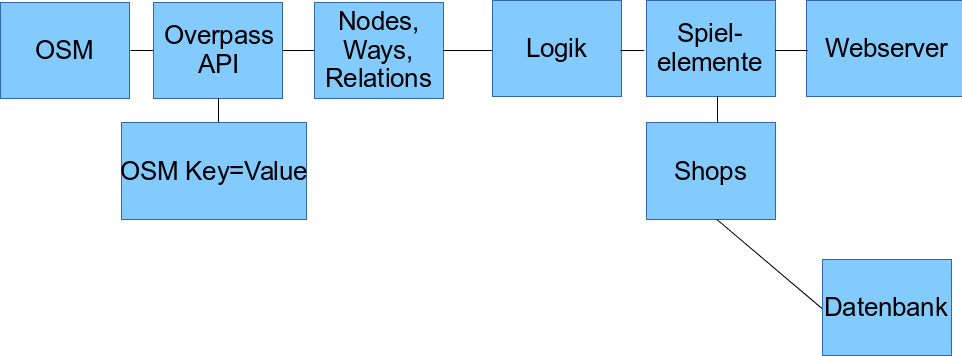
\includegraphics[width=140mm]{images/ch5_img01_framework_progress.png}
\caption{Prozess: Von OSM zum Spielelement}
\label{img:ch5_img01_framework_progress}
\end{center}
\end{figure}

\subsection*{OSM und Overpass API}

Zunächst steht zu Beginn des Prozess als Datengrundlage Openstreetmaps.
Die Daten werden allerdings nicht direkt von OSM über die OSM API abgerufen, sondern über Overpass. Das liegt daran, dass die OSM API selbst nur sehr rudimentäre Abfragen erlaubt.
Stattdessen wird die Overpass API verwendet, da diese geografische Abfragen erlaubt \cite{Meyer.2013}.
Diese Abfragen sind notwendig, um die zuvor deklarierte Anforderung, die Spielelemente basierend auf einem OSM key-value Paars zu bewerkstelligen. Darüber hinaus wird die Transformation der Relations und Ways in Nodes einfacher ermöglicht.
Durch die Verwendung der Overpass QL-Abfrage Sprache (OQL) ist es möglich sich nicht nur die jeweiligen Relations, Ways und Nodes eines tags zu erhalten, sondern auch zusätzlich alle rekursiv enthaltenen Elemente. Dies ermöglicht es den kompletten Datensatz mit einer Abfrage zu erhalten der für die spätere Transformation benötigt wird. Der Vorteil liegt darin, dass nicht mehrere Abfragen gestartet werden müssen und somit die Zeit bis alle Daten zur Verfügung stehen erheblich reduziert wird. Die Overpass API selbst bietet diverse Ausgabe Formate wie XML und JSON \cite{Olbricht.2014}. Für eine konkrete Umsetzung wurde sich bewusst für JSON entschieden, da zum einen die Performance bei der Verabreitung von JSON Dokumenten beachtlich höher ist im Vergleich zu XML Dokumenten \cite{Nurseitov.2009}. Zum anderen soll die Daten später als GeoJSON aufbereitet werden.
Der Aufruf der OverpassAPI erfolgt mittels einfacher REST-Abfrage:
\\\\
\url{http://overpass-api.de/api/interpreter?data=OQL_BEFEHL}
\\\\
Über den Parameter "data" wird der jeweilige OQL Befehl abgesetzt.
Für die Weiterverarbeitung der Daten wird im Anschluss das JSON Ergebnis vom Framework geparst und weiterverarbeitet.

\subsection*{Transformations Logik}

Die Transformation der Relations und Ways wird wie in Kapitel \ref{ch4:s:choosen_solution} umgesetzt. Eine Visualisierung ist in Abbildung \ref{img:ch5_img02_transform} zu sehen.

\begin{figure}[H]
\begin{center}
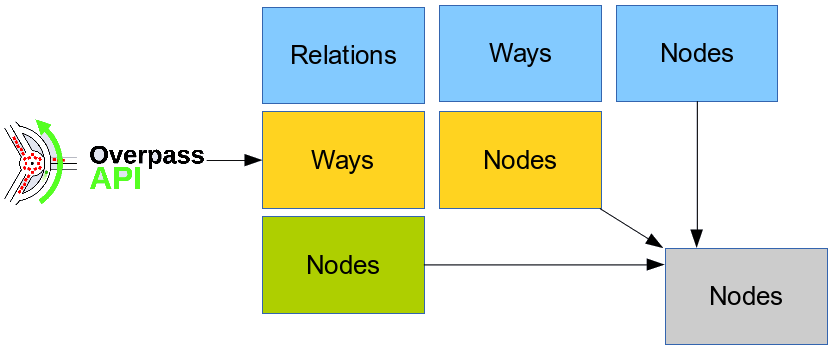
\includegraphics[width=140mm]{images/ch5_img02_transform.png}
\caption{Transformationsprozess: Relations, Ways, Nodes}
\label{img:ch5_img02_transform}
\end{center}
\end{figure}

Auf der linken Seite sind vertikal die Ausgangstypen angeordnet. Hierbei handelt es sich um die bereits angesprochenen Elemente Relations, Ways und Nodes. Im zweiten Schritt, nach dem Aufbereiten der Daten von der Overpass API wird wie folgt vorgegangen. Zunächst werden alle Relations behandelt, im Anschluss darauf die Ways und zum Schluss die Nodes. Die Idee dahinter ist es zunächst alle Ways und Nodes zu identifizieren welche direkt einer Relation angehören und keine separaten Spielelemente darstellen. Die Vorgehensweise ist damit begründet, dass durch die Reduzierung der Anfrage auf ein einzelnen Request die Rückgabe alle Nodes enthält. Sowohl die Nodes einer Relation, als auch die eines Ways, welche selbst nicht eigenständig sind. Daher müssen die Elemente Ebene für Ebene wie in der Abbildung zu sehen, abgearbeitet werden.
\\\\
Zunächst werden alle Relationen identifiziert. Für jede Relation werden nun die beinhalteten Ways und Nodes identifiziert. Diese wiederum werden dann als "gecalaimed" markiert. Relations selbst werden nicht rekursiv aufgelöst, da das Ziel nicht ist möglichst wenige Spielelemente zu haben, sondern Relationen zu transformieren. Sollten Relations mehreren Unterrelations haben so sollen diese als Eigenständige Elemente betrachtet werden. Sofern dieser Ansatz sich als Nachteilig in der Evaluation herausstellt muss er entsprechend modifiziert werden.
Für die jeweilige Iteration eines Relation Elements werden nun alle beteiligten Ways und Nodes zu einer Liste von Nodes zusammengefasst, Diese Liste wird wiederum durch das in Kapitel \ref{ch4:s:choosen_solution} beschriebene Verfahren einer Bounding Box dessen Mittelpunkt berechnet wird reduziert auf ein virtuelles Node, welches die Relation repräsentiert. Dieses virtuelle Node hat eine Koordinate, sowie eine ID welche eindeutig identifizierbar ist. Hierzu wird die Relations ID von OSM verwendet.

Im nächsten Schritt werden die Ways abgearbeitet. Bereits als "geclaimed" markierte Ways, die somit bereits in einer Relation enthalten sind, werden ignoriert. Alle anderen Ways werden entsprechend jeweils wiederum zu einer Liste von Nodes und anschließend zu einem virtuellen Node transformiert. Hierbei entsteht wieder eine Koordinate und als ID wird die OSM Way ID verwendet.

Die Elemente, welche direkt als Node zurückgegeben werden analog übernommen. Sie werden in Spielelemente, hier durch das graue Nodes Element symbolisiert, transferiert. Hierzu wird die Koordinate, sowie die OSM ID der Nodes übernommen.

Eine Problematiks tellt sich allerdings noch in der eindeutigen Identifizierung der virtuellen Nodes. Da diese von unterschiedlichen Elementen (Relatons, Ways, Nodes) abgeleitet wurden muss sichergesteltl werden, dass anhand der ID eine eindeutige OSM Zuordnung möglich ist.
Entweder es wird zusätzlich der abgeleitete typ des Spielelements explizit gespeichert oder aber, man transcodiert die Information mit in die ID.
Wenn man sich zunächst die OSM IDs für Nodes anschaut, stellt man fest, dass diese die 32bit signed Integer Grenze überschritten haben (Februar 2013). Im OSM Wiki wird daher empfohlen den Datentyp long zu verwenden, welcher in den Standard-Implementierungen ein 64bit Wert ist \cite{OSM.2013b}.
Eine Methode um den Typ des Spielelements zu übertragen könnte mit einer Bitmaske der ID funktionieren. Hierzu könnte man die den 2. und 3. Bit Bits des 64bit Wertes verwenden. Der 1. it wird nicht verwendet um negative Zahlen weiterhin zu erlauben. Der 2. Bit würde als Identifikator für Relations dienen und der 3. für Ways als Ursprungselement. Ein Beispiel für den transformierten Way mit der OSM ID 1 ist in Abbildung \ref{img:ch5_img03_bitmask} zu sehen.

\begin{figure}[H]
\begin{center}
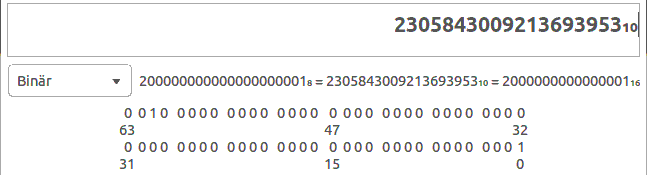
\includegraphics[width=120mm]{images/ch5_img03_bitmask.png}
\caption{OSM ID: Bitmaskenkodierung im 64bit long Wert}
\label{img:ch5_img03_bitmask}
\end{center}
\end{figure}


Wenn man die Reduzierung von 63bit (signed) auf 61bit(signed) mit der aktuellen Mapping Geschwindigkeit bei OSM vergleicht, so lässt sich feststellen, dass die Reduzierung um 2 bit aus Paradigmensicht zwar unsauber erscheint, aber eine Überschreitung der ID \begin{math}2^{61}\end{math} in ferner Zukunft liegt. Zudem könnte im Bedarfsfall wenn OSM auf 128bit IDs umsteigt die Bitmaske entsprechend angepasst werden.

\subsection*{Händler Integration}

Nachdem die virtuellen Nodes für die Spielelemente alle erstellt wurden, müssen die Elemente um die Händlern ergänzt werden. In Kapitel \ref{ch4:s:choosen_solution} wurde erläutert, dass die Händler nicht als aktives Spielzielelement verwendet werden sollen, sondern eine Integration der Händler und Dienstleister im Spiel als Repräsentation ihrer Selbst. Die Händler fungieren in diesem Zusammenhang als Anbieter für Items und andere Gegenstände. Für die spätere Darstellung auf der Karte müssen diese ebenfalls mit einer Koordinate versehen werden und separat behandelt werden. D.h. die Spielpunkte der Händler kommen stattdessen aus einer lokalen Datenbank. Dabei wird bewusst auf die Verwendung von OSM Als Basis verzichet. Zwar könnte man in einer erweiterten Version des Frameworks dem Nutzer unterstützen mit automatischen Vorschlägen basierend auf OSM, jedoch ist dies in der Grundfunktion nicht notwendig. Hier soll der Händler sich beliebig frei auf der Karte Positionieren können und entsprechende Parameter seines virtuellen Geschäfts festlegen. Im Anschluss soll er entsprechende Items in seinem virtuellen Shop hinterlegen können. Da die Items eventuell vom Händler gegen einen Betrag vom Spielleiter erkauft werden, hat der Spielleiter ein gewisses Interesse, dass er zum einen die Items im Spiel möglichst an die Spieler bringt, während er auf der anderen Seite das Spiel nicht in einen nicht balancierten Zustand bringt. D.h. dass eventuell zu viele Spieler durch die Nähe eines Händlers mit einem sehr nützlichen Item bevorzugt werden. Daher sollte es im Ermessen des Spielleiters liegen, dass dieser die Art und Verwendung der Items selbst definiert und entsprechende Vorschläge für die Händler parat hat. Dass der Händler selbst sich mit Spielmechaniken und Balancing auseinander setzt ist höchst unwahrscheinlich und würde auch nur zu extra Koordinationsaufwand führen. Daher ist es am sinnvollsten dem Händler gewisse Items mit standard Eigenschaften anzubieten, von denen er einen Typ selbst auswählt und eine entsprechende Menge seinem virtuellen Shop zuordnet.
Für die Itemtypen kann der Spielleiter aller Voraussicht nach auf gewisse Grunderfahrungen zurückgreifen. Darüber hinaus sollte das Framework ihm zu einem späteren Zeitpunkt in einer erweiterten Ausbauphase auch entsprechendes Feedback über die Verwendung und Nutzung der Items aufzeigen und der Spielleiter somit aufgrund dieser Information Rückschlüsse auf das Balancing machen kann.

\subsection*{Persistenz}

Ein wichtiger Aspekt des Frameworks stellt die Persistenz dar. Zum einen müssen die Spielelemente als auch der Spielzustand selbst gespeichert werden.


\subsection*{Schnittstellen}

\subsection*{Spiel Darstellung}

\subsection*{Softwaretechnischer Entwurf}

\section{Bewertung der Technologien und Werkzeuge}

\section{Implementierung des Geogameframeworks}